\documentclass[9pt,twocolumn,twoside,lineno]{pnas-new}
% Use the lineno option to display guide line numbers if required.
% Note that the use of elements such as single-column equations
% may affect the guide line number alignment. 

\templatetype{pnasresearcharticle} % Choose template 
% {pnasresearcharticle} = Template for a two-column research article
% {pnasmathematics} = Template for a one-column mathematics article
% {pnasinvited} = Template for a PNAS invited submission


\usepackage{comment}
\usepackage[capitalize]{cleveref}
\usepackage{graphicx}

\graphicspath{{./}{figures/}}

\newcommand{\figcaption}[1]{\refstepcounter{figure} \subsection*{Fig. \thefigure{}} #1}
\newcommand{\tabcaption}[1]{\refstepcounter{table}}


\title{Blind-dating: recovering the integration dates of the latent human immunodeficiency virus reservoir using longitudinal samples}

% Use letters for affiliations, numbers to show equal authorship (if applicable) and to indicate the corresponding author
\author[a]{Bradley R. Jones}
\author[b]{Natalie N. Kinoch} 
\author[a]{Joshua Horacsek}
\author[b]{Philip Mwimanzi}
\author[b]{Bemuluyigza Baraki}
\author[c]{John Huang}
\author[c]{Ronald Truong}
\author[a]{Bruce Ganase}
\author[a]{Marianne Harris}
\author[a]{Robert Hollebakken}
\author[a,d]{P. Richard Harrigan}
\author[c]{R. Brad Jones}
\author[a,b]{Mark A. Brockman}
\author[a,d,1]{Jeffrey B. Joy}
\author[e,1]{Art F. Y. Poon}
\author[b,1,2]{Zabrina L. Brumme}

\affil[a]{BC Centre for Excellence in HIV/AIDS, 608-1081 Burrard St Vancouver, Canada V6Z 1Y6}
\affil[b]{Faculty of Health Sciences, Simon Fraser University, 8888 University Drive
Burnaby, Canada V5A 1S6}
\affil[c]{Department of Microbiology, Immunology and Tropical Medicine, George Washington University, Ross Hall 2300 Eye Street, NW, Suite 502 Washington, DC, United States of America 20037}
\affil[d]{Department of Medicine, University of British Columbia, 2775 Laurel Street, 10th Floor
Vancouver, Canada V5Z 1M9}
\affil[e]{Department of Pathology and Laboratory Medicine, Western University, Dental Sciences Building, Rm. 4044
London, Canada N6A 5C1}

% Please give the surname of the lead author for the running footer
\leadauthor{Jones} 

% Please add here a significance statement to explain the relevance of your work
\significancestatement{Significance (120 words).}

% Please include corresponding author, author contribution and author declaration information
\authorcontributions{J.B.J., A.F.Y.P., Z.L.B. conceived and designed the experiments. P.R.H., Z.L.B. procured the materials. N.N.K., R.H., Z.L.B. processed the materials. B.R.J., J.H. wrote the software. B.R.J., J.B.J, A.F.Y.P., Z.L.B. performed the analysis. B.R.J., J.B.J, A.F.Y.P., Z.L.B. wrote the maunscript.}
\authordeclaration{Please declare any conflict of interest here.}
\equalauthors{\textsuperscript{1}J.B.J.(Jeffrey B. Joy), A.F.Y.P. (Art F. Y. Poon), and Z.L.B (Zabrina L. Brumme) contributed equally to this work.}
\correspondingauthor{\textsuperscript{2}To whom correspondence should be addressed. Address: Faculty of Health Sciences, Simon Fraser University, 8888 University Drive
Burnaby, Canada V5A 1S6, Telephone: +1-778-782-8872, Email: zbrumme@sfu.ca}

% Keywords are not mandatory, but authors are strongly encouraged to provide them. If provided, please include two to five keywords, separated by the pipe symbol, e.g:
\keywords{Human immunodeficiency virus $|$ Viral reservoirs $|$ Phylogenetics $|$ Linear models} 

\begin{abstract}
Here we present a method to recover the insertion dates of integrated proviral human immunodeficiency virus.
\end{abstract}

\dates{This manuscript was compiled on \today}
\doi{\url{www.pnas.org/cgi/doi/10.1073/pnas.XXXXXXXXXX}}

\begin{document}

% Optional adjustment to line up main text (after abstract) of first page with line numbers, when using both lineno and twocolumn options.
% You should only change this length when you've finalised the article contents.
\verticaladjustment{-2pt}

\maketitle{}
\thispagestyle{firststyle}
\ifthenelse{\boolean{shortarticle}}{\ifthenelse{\boolean{singlecolumn}}{\abscontentformatted}{\abscontent}}{}

% If your first paragraph (i.e. with the \dropcap) contains a list environment (quote, quotation, theorem, definition, enumerate, itemize...), the line after the list may have some extra indentation. If this is the case, add \parshape=0 to the end of the list environment.
\dropcap{H}IV-1, like all retroviruses, integrates its genome into the chromosome of the infected host cell during the viral life cycle.
Though the vast majority of infected cells die as a result of viral cytopathic effects or immune-mediated elimination, a small minority (broadly estimated as one in every million resting CD4+ T-cells \cite{Chun97,Finzi97}) harbour integrated HIV DNA in a state of near or complete transcriptional quiescence over long time periods \cite{Archin14,Pace11,Richman09}.
Termed latent HIV-1 reservoirs, such cells represent a major obstacle in curing HIV-1 infection as they can persist for years.
In the presence of suppressive antiretroviral therapy, for instance, these reservoirs can be re-activated at any point to produce infectious virus, thereby reseeding infection \cite{Richman09,Durand12,Joos08,Katlama13,Pomerantz03,Shen08}. 

Establishment of individual viral reservoirs within a given host  begins within hours or days following infection and continues thereafter \cite{Whitney14,Leford14}.
As within-host HIV-1 populations rapidly accumulate genetic diversity over the course of an infection \cite{Alizon13,Rambaut04,Shankarappa99}, latent viral genomes present during untreated chronic infection should be heterogeneous in terms of age and genetics, ranging from those archived soon after infection (that resemble ancestral viruses within the host) to those that have integrated relatively recently into cellular reservoirs (that resemble contemporary plasma strains).
The chronology of establishment and genetic distribution of latent HIV-1 lineages within a given host is may be relevant to the development of strategies to eliminate them, as these properties could influence their susceptibility to reactivation and/or immune-mediated clearance.
For example, while the `oldest' reservoirs within a given individual may be the most inherently refractory to reactivation with latency reversing agents, `younger' reservoirs may be largely refractory to subsequent immune-mediated elimination due to an accumulated burden of immune escape mutations \cite{Deng15}.
However, within-host dynamics of HIV-1 reservoir establishment remain incompletely characterized.
Previous studies have developed techniques to detect latent lineages by reduced rates of viral evolution \cite{Immonen14} and modelled the population dynamics of different classes of the virus within a given host \cite{Althaus14}.
However, there has been limited research on estimating when known or suspected latent viral lineages originally became integrated into their respective host cell genomes, or qualitatively assessing the age distributions of latent HIV-1 lineages within a given host.  

We here describe a novel phylogenetic method to `date' individual viral reservoir sequences within a host.
The method utilizes longitudinal plasma HIV RNA sequences sampled over an individual's infection to calibrate a host-specific HIV evolutionary rate from which the ages of known or suspected reservoir sequences are then inferred. The premise is as follows.
Because HIV-1 sequences within a given infected host rapidly accumulate genetic diversity due to HIV-1's high mutation rate and short generation time \cite{Alizon13,Rambaut04,Shankarappa99}, it is possible to reconstruct a phylogenetic tree that represents the ancestor-descendant relationships between HIV-1 sequences sampled longitudinally from within that host.
A phylogeny that is reconstructed by parametrizing a model of molecular evolution solely on the basis of sequence homology (\emph{e.g.}, by maximum likelihood estimation \cite{Felsenstein81}) has branch lengths in units of expected numbers of substitutions, in which the passage of time is confounded with the rate of evolution.
In other words, a tree that stretches far back in time with a slow rate of evolution will explain a given set of sequences just as effectively as a shallow tree with rapid evolution.
When sampling dates are known however, the corresponding tips of the phylogeny can be fixed at these time points, allowing the rate of evolution to be estimated directly \cite{Rodrigo99}.
Knowledge of sampling dates thus enables one to rescale a phylogeny in chronological time, which is especially useful for within-host HIV-1 populations in which substantial genetic differences can accumulate in weeks or months \cite{Williamson03}.
Moreover, among the actively replicating HIV lineages within a host, the rate of molecular evolution is fairly consistent over time \cite{Korber00,Kuhner95,Leitner99,Park16}.
Consequently, the divergence of descendant lineages from the transmitted/founder virus can be approximated by a `strict' molecular clock model in which a consistent rate of evolution is sustained, at least over the initial years, of an individual's infection course \cite{Keele08}. 

Upon integration of a given HIV-1 sequence into a host cell genome, evolution of that lineage effectively ceases until a new round of virus replication ensues.
Latent HIV-1 sequences will therefore display a characteristic discordance between their sampling date and their apparent (younger) age based on sequence divergence from other within-host lineages.

We validated our method on simulated phylogenies.
Then we applied our method to patient data from a patient with longitudinal RNA plasma-derived sequences while treatment-naive and DNA PBMC-derived sequences after the patient recieved anitretroviral theray for 6--10 years.
We compared results of using single-genome amplification and next-generation sequencing of the NEF and V3 regions respectively.

\section*{Reconstructing integration dates}
Since HIV evolution adheres to the molecular clock hypothesis \cite{Leitner99,Park16}, the genetic distance of virions from the founder virus is linear with respect to time.
However, while under viral latency, the virus does not replicate and hence does not evolve, essentially stopping the molecular clock.
Hence, the date of the insertion of provirial insertion is when the molecular clock stops and is linearly related to the genetic distance of the proviral sequence to the founder virus.
See \cref{fig:latenttree}.

\begin{figure}
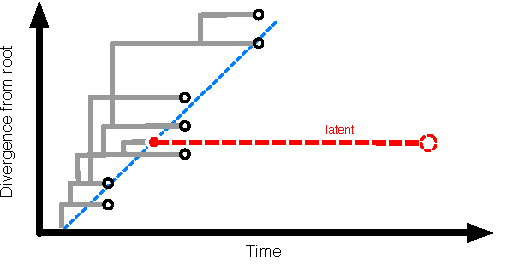
\includegraphics{latency-scheme}
\caption{Reconstructing the time that a viral lineage entered a latent state from with-host sequence variation.
	A dashed line illustrates the linear relationship between the divergence of lineages from the ancestral sequence at the root ($y$-axis) and passage of time since the root ($x$-axis).
	Grey lines represent the reconstructed phylogenetic relationships among these lineages.
	The lineages were sampled (open circles) at three points in time.
	One of these lineages had become latent at an earlier point in time (red hexagon).
	This lineage subsequently underwent negligible molecular evolution until it was sampled as integrated viral DNA (dashed circle).
	If the relationship between sequence divergence and time is sufficiently linear, then the time between latency establishment and sampling, here represented by the thick red dashed line, can be inferred from its sequence.
}
\label{fig:latenttree}
\end{figure}

The model resets on the reconstruction the phylogenetic relationships of longitudinaly-sampled HIV sequences.
A phylogenetic tree can be created using a variety of methods including neighbour-joining \cite{Saitou87}, maximum likelihood \cite{fasttree,raxml}, Bayesian methods ((possible footnote)) \cite{beast}, \emph{et cetera}.
After assigning a root to the phylogeneteic tree (using outgroup rooting  \cite{Huelsenbeck02}, root-to-tip regression  \cite{Korber00}, \emph{et cetera}), we recover the linear molecular clock with a linear model (LM).
Our LM is given by:
\begin{align}
	D &= a + \mu T,\label{eq:glm}
\end{align}
with response: $D$, the genetic distance from the root of the tree; predictor: $T$, the collection date; and parameters: $\mu$, the mutation rate and $a$, a genetic distance shift.
First we censor the provial DNA sequences and use the virion RNA sequences to calibrate the LM.
Next we recover the provial insertion dates by computing $T(x) = \frac{D(x) - a}{\mu}$, for each proviral DNA sequence, $x$.
Details of the method are given in the Materials and Methods.

\section*{Model validation on simulated data}
To validate our method, we tested its performance on simulated phylogenies --- see the Materials and Methods for details on their construction.


\section*{Patient data}

\subsection*{Nef sequences}
The blind-dating methods were applied to HIV sequences from the NEF region retrived using single-genome amplification.

The correlation between the estimated dates for our patient using the different rooting methods --- outgroup rooting (OGR) and root-to-tip regression (RTT) --- was 0.95 (pearson)/0.94 (spearman) and the root mean square deviation was 540 days.
RTT optimizes the molecular clock and linear regression, where OGR is more biological motivated, therefore the high correlation is promising.
See \cref{fig:nefdistvtime} for a comparison of the two rooting methods.

\begin{figure*}
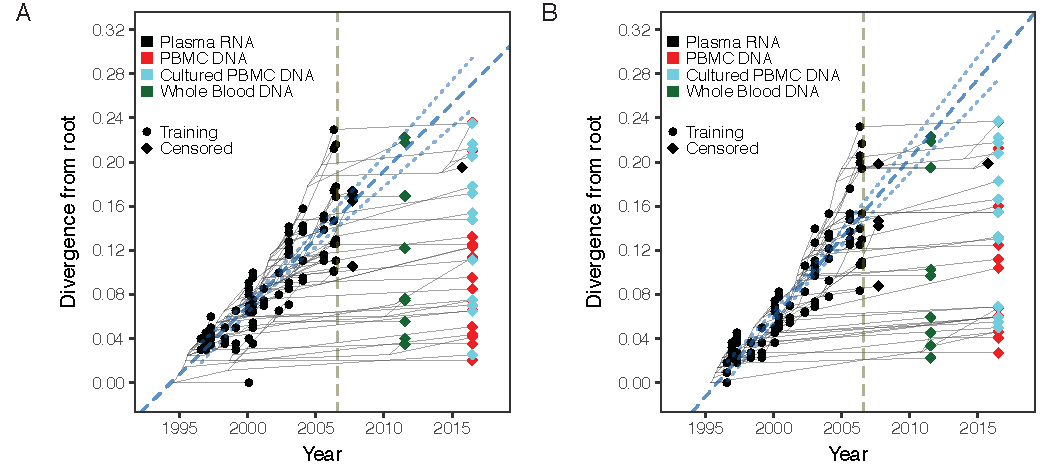
\includegraphics{nefdistvtime}
\caption{The distance from the root versus time.
(A) OGR (B) RTT.}
\label{fig:nefdistvtime}
\end{figure*}

\subsection*{V3 sequences}
The blind-dating methods were also applied to HIV sequences from the V3 region retrived using deep sequencing.

The correlation between the estimated dates for our patient using the different rooting methods --- outgroup rooting (OGR) and root-to-tip regression (RTT) --- was 0.95 (pearson)/0.84 (spearman) and the root mean square deviation was 270 days.
See \cref{fig:v3distvtime} for a comparison of the two rooting methods.

\begin{figure*}
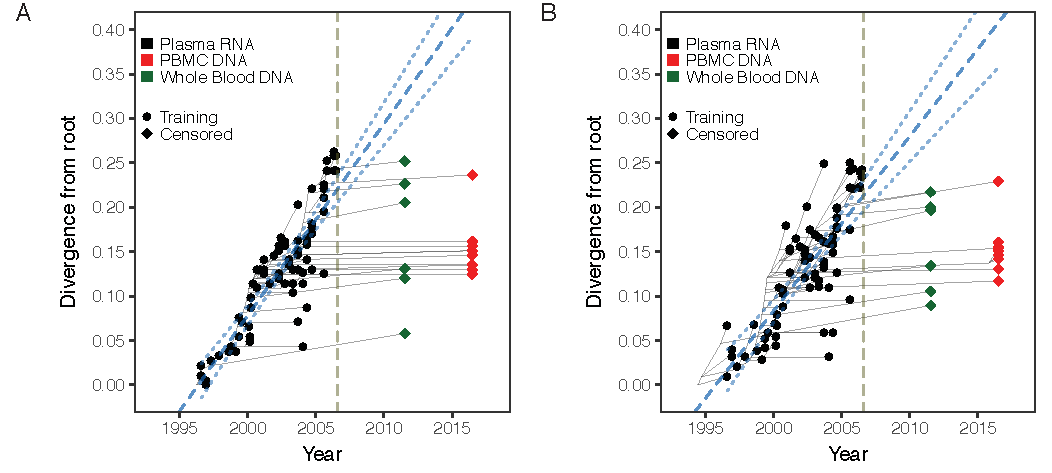
\includegraphics{v3distvtime}
\caption{The distance from the root versus time.
(A) OGR (B) RTT.}
\label{fig:v3distvtime}
\end{figure*}

\subsection*{Sensitivity testing}
We reduced the patient data set of the NEF data set to quantify the effect of the number of time points used.
The NEF data set had 14 time points with training RNA sequences.
We reduced the patient data by selecting a subset of the 14 time points at random.
From this we generated 550 different data sets with 2--12 time points with training RNA sequences (50 data sets for each number of time points) and all 14 possible data sets with 13 time points of training RNA sequences.
We applied the blind-dating methodology to each data set.

\begin{figure*}
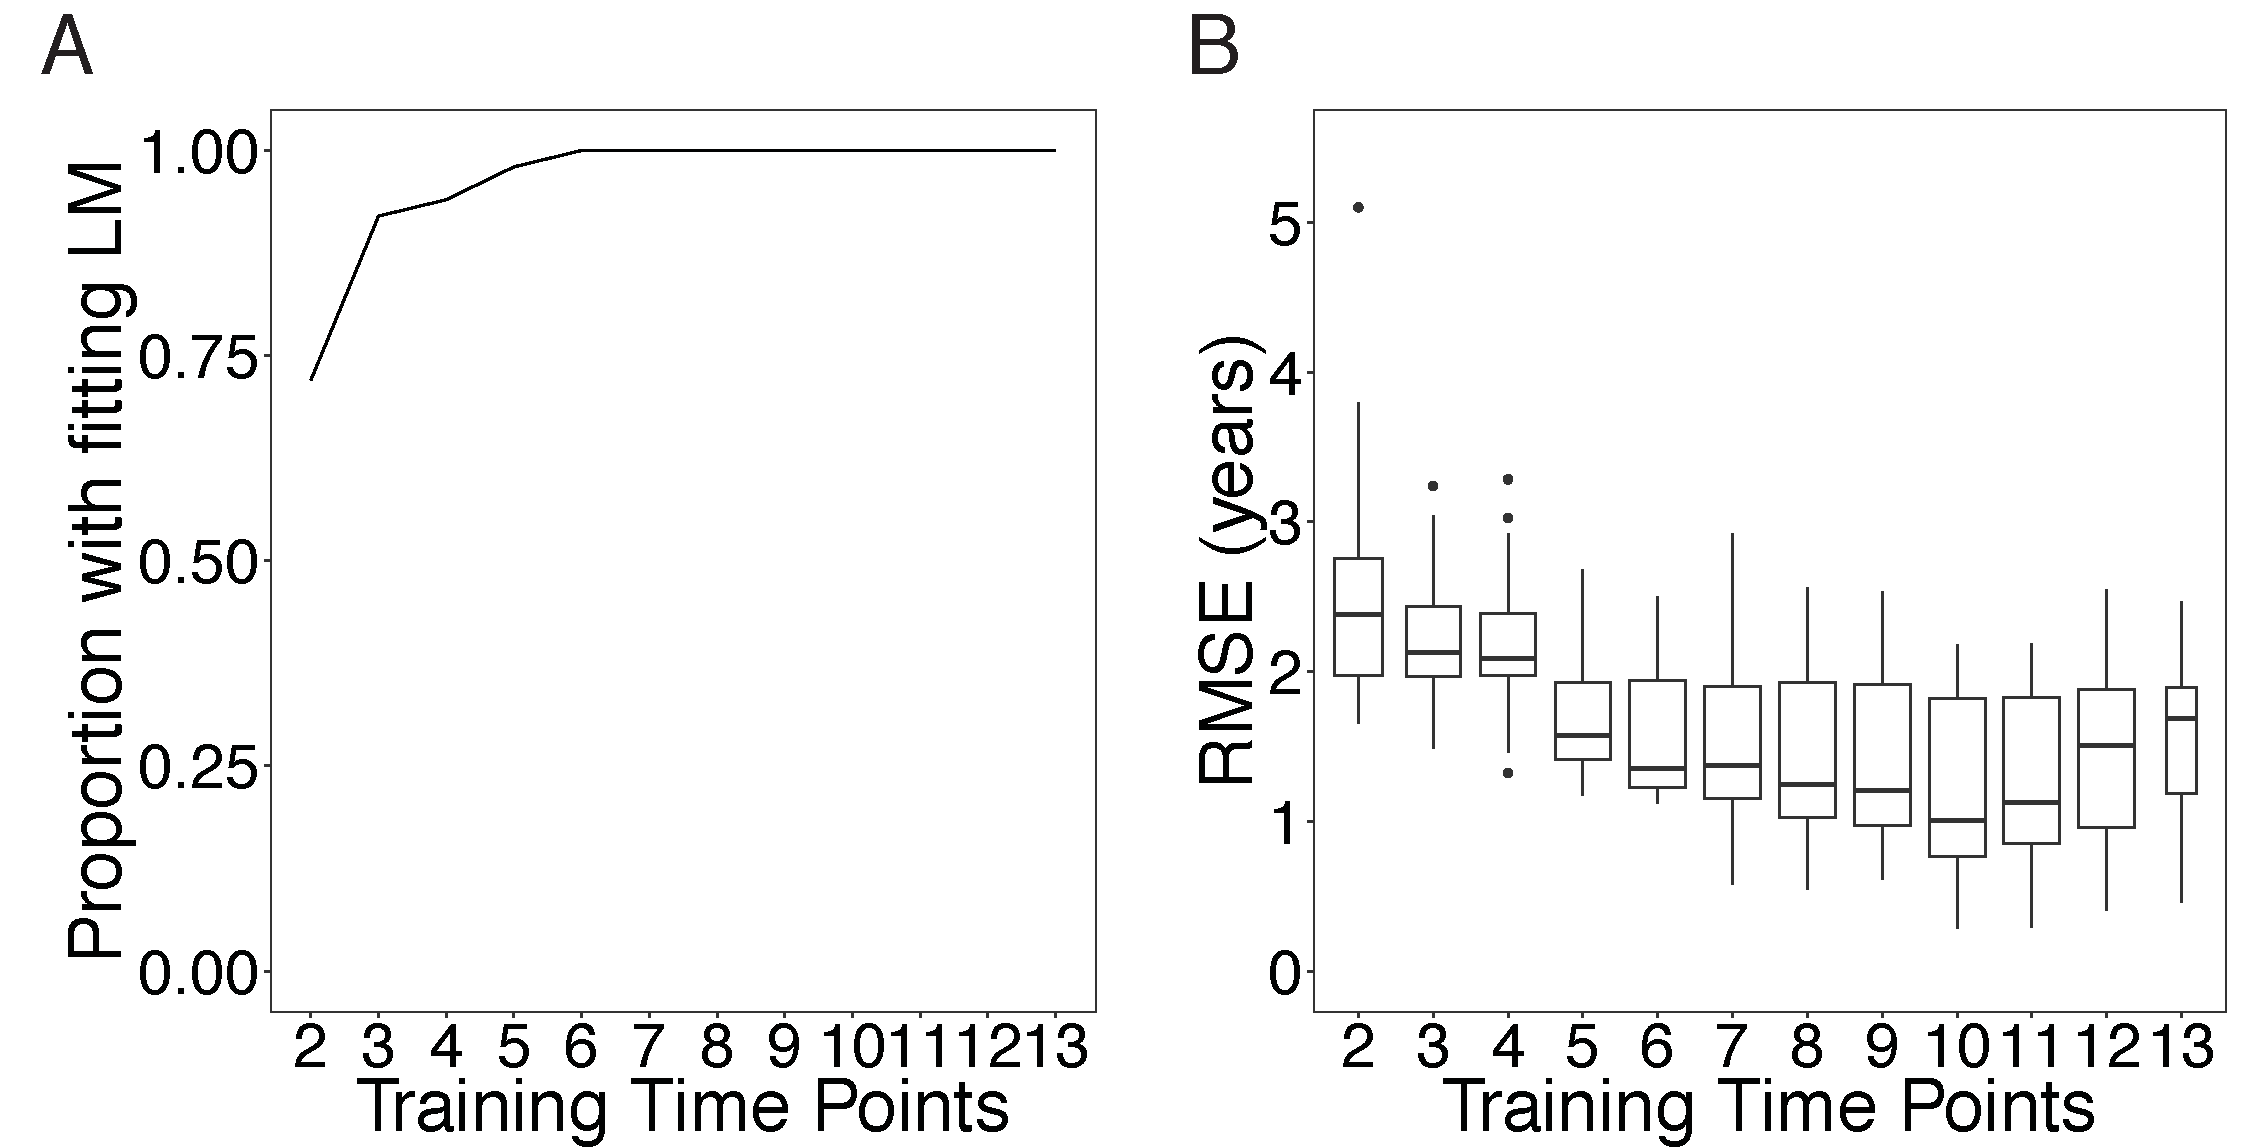
\includegraphics{sensitivity}
\caption{The root mean squared error.
(A) OGR (B) RTT.}
\label{fig:sensrmse}
\end{figure*}

\section*{Conclusions}
((Short conclusion)).

((Limitations))

Patient viral load.

Requires longitudinal data.

HIV doesn't strictly follow a molecular clock and evolution under treatment is poorly understood.

((Wrap up))

Most other models of HIV latent reservoirs are dynamical models \cite{Rong09,Pace11}. These models can be complicated, including many components and parameters.



\matmethods{
\subsection*{Data collection, sequencing and alignment}
((Collection/Ethics/Metadata.))
((Sequencing.))
((Check for recombination/hypermutation.))
The sequences were aligned using MUSCLE v3.8.31 \cite{muscle} and inspected and cleaned with AliView v1.18 \cite{aliview}.
For each pair of identical sequences, we retained only one copy.
There was one instance where there was a triplet of RNA sequences that were collected at two different time points.
For this triplet we kept one sequence from the earlier time point.
\subsection*{Simulated data generation}
To characterize sources of error in reconstructing dates on tips of a phylogeny, we generated phylogenetic trees by direct simulation.
We generated phylogenies with 50 tips each under a birth-death model with serial sampling using the sim.bdsky.stt function in the R package TreeSim v2.3.
We estimated the parameters to use for the birth-death model by fitting the HIV RNA sequences from Patient ***REMOVED*** (except for the sequence from 2015 `viremia blip') to the birth-death serially sampled model in BEAST v1.8.3 \cite{beast} using $10^9$ runs including $10^8$ runs of burn-in.
This gave us birthrate: $\lambda = 8.87 \times 10^{-7}$ day${}^{-1}$, death rate: $\delta = 7.75 \times 10^{-3}$ day${}^{-1}$, and sampling proportion: $s = 0.115$.
We applied a molecular clock to the generated phylogenies using the R package NELSI v \cite{nelsi} with mean rate $4.03 \times 10^{5}$ substitutions per base per day and standard deviation $1.84  \times 10^{-6}$ substitutions per base per day.
These values were obtained from estimated paramater value and standard deviation of $\mu$ in the linear model (LM) given in \cref{eq:glm} using R \cite{rscript}.
Finally, we created simulated HIV RNA sequences from these phylogenies with INDELible v1.03 \cite{indelible}, to create one set of 50 simulated HIV RNA sequences per phylogeny.
We applied the blind-dating methodology to each simulated data set.
\subsection*{Blind-dating}
We reconstructed the within-host phylogenies of each subject in each data set as maximum likelihood phylogenies reconstructed using RAxML v8.2.4 \cite{raxml} with the GTR model.
We evaluated two different methods for rooting these trees. 
The first method was outgroup rooting (OGR), in which one or more sequences from taxa outside but sufficiently related to the group of interest are added to the phylogenetic reconstruction \cite{Huelsenbeck02}.
The point at which the branch leading to the outgroup intersects the rest of the tree provides an estimate of the root for the latter.
We selected the HIV-1 B ancestral sequence reconstruction,  curated by the LANL HIV sequence database as the outgroup sequence.
The second method was root-to-tip regression (RTT) \cite{Korber00}, which performs an exhaustive search by re-rooting the tree at every branch to find the root that (in our experiments) maximizes the correlation between the sample collection dates and the evolutionary distance of tips from the candidate root.
Our simulated data were only rooted using RTT; for all real data, both outgroup rooting and RTT were evaluated for rooting the phylogeny.
For each subject in each data set, we computed the LM given in \cref{eq:glm} using the R function, lm \cite{rscript}.
\subsection*{Statisical Analysis}
((Methods used)).
All statistical calculations were performed using R \cite{rscript}.
All plots were generated using the ggplot2 and ggtree packages in R \cite{ggplot,ggtree} --- time-scaled versions of the trees were generated using the esimate.dates function of the ape package in R \cite{ape,nodedating}.
}

\showmatmethods{} % Display the Materials and Methods section

%\acknow{Ack}

%\showacknow{} % Display the acknowledgments section

% \pnasbreak splits and balances the columns before the references.
% If you see unexpected formatting errors, try commenting out this line
% as it can run into problems with floats and footnotes on the final page.
\pnasbreak{}

% Bibliography
\bibliography{blind-dating}
\end{document}


%% Do not use widetext if paper is in single column.
\begin{widetext}
\begin{align*}
(x+y)^3&=(x+y)(x+y)^2\\
       &=(x+y)(x^2+2xy+y^2) \numberthis \label{eqn:example} \\
       &=x^3+3x^2y+3xy^3+x^3. 
\end{align*}
\end{widetext}

\begin{table}%[tbhp]
\centering
\caption{Comparison of the fitted potential energy surfaces and ab initio benchmark electronic energy calculations}
\begin{tabular}{lrrr}
Species & CBS & CV & G3 \\
\midrule
1. Acetaldehyde & 0.0 & 0.0 & 0.0 \\
2. Vinyl alcohol & 9.1 & 9.6 & 13.5 \\
3. Hydroxyethylidene & 50.8 & 51.2 & 54.0\\
\bottomrule
\end{tabular}

\addtabletext{nomenclature for the TSs refers to the numbered species in the table.}
\end{table}